\section{Princípios de Arquitetura Limpa}
    \subsection{Contexto histórico}
        \par A Arquitetura Limpa foi proposta por Robert C. Martin em 2012, conforme publicado no blog The Clean Code Blog \cite{artigo:ferreira:2022}. A abordagem foi desenvolvida com base em sua experiência como programador desde 1970 \cite{livro:martin:cleanarch}.
        
        \par O surgimento da Arquitetura Limpa está associado à "crise do software" da década de 1960, caracterizada por problemas como prazos não cumpridos, custos elevados, baixa produtividade, qualidade insuficiente e dificuldades de manutenção em aplicações \cite{artigo:dantas:2021, artigo:ferreira:2022}. Essa crise evidenciou a necessidade de métodos para gerenciar a complexidade e os custos de manutenção de software \cite{livro:martin:cleanarch}.

        \par A partir dos anos 1970, estudos e pesquisas buscaram melhorar os processos de desenvolvimento, resultando no avanço de ferramentas, métodos, padrões e técnicas para a criação de software de qualidade \cite{artigo:dantas:2021}. A Arquitetura Limpa foi concebida para promover sistemas organizados, testáveis e escaláveis, atendendo às demandas de desenvolvimento colaborativo e entrega contínua em contextos empresariais e acadêmicos \cite{artigo:ferreira:2022}.
        
    \subsection{Definição}

        \par A Arquitetura Limpa é um conjunto de princípios e práticas de design de software proposto por Robert C. Martin, com o objetivo de criar sistemas manuteníveis, escaláveis e testáveis, priorizando a separação de responsabilidades e a independência de detalhes técnicos \cite{livro:martin:cleanarch}.

        \par A arquitetura limpa define que o sistema deve ser estruturado em camadas concêntricas, com as regras de negócio (entidades) no centro e os detalhes técnicos (frameworks, bancos de dados) na periferia, seguindo a Regra da Dependência ao qual vamos explicar mais a frente neste trabalho e estabelecendo que as dependências do código-fonte devem apontar para as camadas internas, garantindo o desacoplamento entre camadas \cite{livro:martin:cleanarch}.

    \subsection{Conceitos Fundamentais}
        \subsubsection{Paradigmas de Programação}

            \par Os paradigmas de programação são a base para a implementação da Arquitetura Limpa, fornecendo estruturas para organizar o código de forma previsível e manutenível \cite{livro:martin:cleanarch}. A literatura destaca três paradigmas principais para aplicação da arquitetura limpa:

            \begin{itemize}
                \item Programação Estruturada: Introduzida por Edsger Dijkstra, elimina o uso indiscriminado de comandos goto, utilizando estruturas como sequências, seleções e iterações para garantir maior controle e previsibilidade no fluxo do programa. Este paradigma é essencial para a construção de algoritmos claros e testáveis \cite{livro:martin:cleanarch}.

                \item Programação Orientada a Objetos (POO): Baseada nos conceitos de encapsulamento, herança e polimorfismo, a POO permite a criação de componentes modulares e reutilizáveis. O polimorfismo, em particular, é crucial para a aplicação da inversão de dependências, possibilitando que camadas internas sejam independentes de detalhes técnicos externos \cite{livro:martin:cleanarch}.

                \item Programação Funcional: Valoriza o conceito de imutabilidade dos dados e a segregação de estados mutáveis, reduzindo efeitos colaterais e aumentando a confiabilidade do sistema. Este paradigma é aplicado em casos de uso que exigem alta previsibilidade \cite{livro:martin:cleanarch}.
                
            \end{itemize}

        \subsection{Princípios SOLID}
            \par Os princípios SOLID foram consolidados por Robert C. Martin na década de 1990, são diretrizes de design orientado a objetos que promovem modularidade, extensibilidade e manutenibilidade \cite{livro:martin:cleanarch}. Esses princípios são fundamentais para a Arquitetura Limpa pois garantem que as camadas do sistema sejam coesas, desacopladas e independentes de detalhes técnicos \cite{livro:martin:cleanarch}. 
            
            \par Cada princípio é descrito abaixo, com sua aplicação e exemplos práticos.

            \subsubsection{Princípio da Responsabilidade Única (Single Responsibility Principle - SRP)}
                \par O SRP estabelece que uma classe deve ter apenas uma razão para mudar, encapsulando uma única responsabilidade perante um ator específico \cite{livro:martin:cleanarch}. Na Arquitetura Limpa, o SRP é aplicado para separar responsabilidades entre camadas, como entidades (regras de negócio genéricas) e casos de uso (fluxos específicos), reduzindo a complexidade \cite{livro:martin:cleanarch}. 
                
                \par Por exemplo, no projeto SmartEye \cite{artigo:dantas:2021}, a classe User gerencia apenas atributos como id e email, enquanto a lógica de autenticação é delegada a outra classe, garantindo coesão. O SRP facilita testes unitários e refatorações, como demonstrado por \cite{inproceedings:nugroho:2022}, que reduziu a duplicação de código em um projeto Laravel.

            \subsubsection{Princípio Aberto/Fechado (Open/Closed Principle - OCP)}

                \par O OCP determina que classes devem ser abertas para extensão, mas fechadas para modificação, assim permitindo a adição de funcionalidades sem alterar o código existente \cite{livro:martin:cleanarch}. Na Arquitetura Limpa, o OCP é implementado por meio de interfaces e herança, especialmente em adaptadores, para suportar novas integrações \cite{livro:martin:cleanarch}. 

            \subsubsection{Princípio da Substituição de Liskov (Liskov Substitution Principle - LSP)}

                \par O LSP estabelece que objetos de uma classe derivada devem ser substituíveis por objetos de sua classe base sem alterar o comportamento do sistema. Na Arquitetura Limpa, o LSP garante consistência em hierarquias de classes, como nas entidades e adaptadores, permitindo substituições seguras \cite{livro:martin:cleanarch}.

            \subsubsection{Princípio da Segregação de Interface (Interface Segregation Principle - ISP)}
            
                \par O ISP determina que classes não devem implementar métodos de interfaces que não utilizam, promovendo interfaces específicas \cite{livro:martin:cleanarch}. Na Arquitetura Limpa, o ISP é aplicado nos limites entre camadas, garantindo interfaces coesas \cite{livro:martin:cleanarch}.
                
            \subsubsection{Princípio da Inversão de Dependência (Dependency Inversion Principle - DIP)}
            
                \par O DIP estabelece que os módulos de alto nível não devem depender de módulos de baixo nível, mas ambos devem depender de abstrações \cite{livro:martin:cleanarch}. Na Arquitetura Limpa, o DIP é a base da Regra da Dependência, garantindo que camadas internas sejam independentes de frameworks externos \cite{livro:martin:cleanarch}. O DIP aumenta a flexibilidade e testabilidade, reduzindo custos de manutenção \cite{artigo:dantas:2021}.
            
    \subsection{Componentes da Arquitetura Limpa}
        \par A Arquitetura Limpa busca organizar o sistema em camadas concêntricas, ou seja, com dependências apontando para dentro, conforme a Regra da Dependência. As camadas incluem entidades, casos de uso, adaptadores de interface, frameworks e drivers, conectados por limites que garantem desacoplamento \cite{livro:martin:cleanarch}.
        
        \par Abaixo segue a explicação para cada um desses conceitos, que são a base para o entendimento da arquitetura limpa.

         \begin{figure}[H] % O [H] exige o uso do pacote float (veja abaixo)
            \centering
            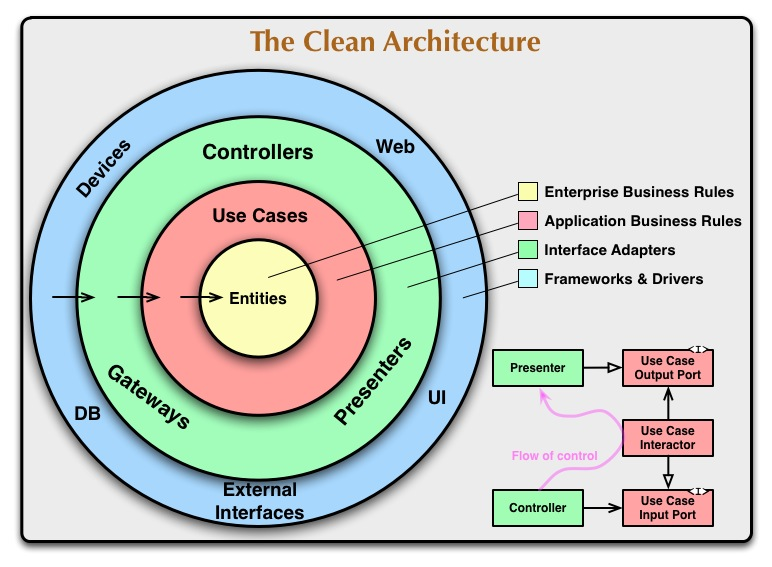
\includegraphics[width=0.8\textwidth]{figuras/clean_arch_1.jpg}
            \caption{A arquitetura limpa}
            \label{fig:figura_clean_arch_1}
            \newcommand{\source}{Fonte: \cite{livro:martin:cleanarch}}
        \end{figure}
        
        \subsubsection{Regra da Dependência}
            \par A Regra da Dependência estabelece que dependências do código-fonte devem apontar para camadas internas, garantindo que nada em uma camada externa seja conhecido pelas camadas internas, incluindo funções, classes ou formatos de dados (Martin, 2020, p. 26; Nugroho, 2022, p. 2; Dantas et al., 2021, p. 5). Essa regra é implementada por meio de interfaces abstratas, que isolam as camadas internas (entidades e casos de uso) de detalhes técnicos externos, como bancos de dados ou frameworks (Martin, 2020, p. 226). No projeto SmartEye, a camada de casos de uso não conhece as implementações de adaptadores, como o banco de dados específico, respeitando a Regra da Dependência (Dantas et al., 2021, p. 6). Isso promove flexibilidade e facilita substituições de tecnologias.


        \subsubsection{Entidades}
            \par As entidades encapsulam regras de negócio genéricas da empresa, sendo objetos ou coleções de dados e funções independentes de tecnologias externas (Martin, 2020, p. 226; Ferreira et al., 2022, p. 6; Dantas et al., 2021, p. 5). Elas formam a camada central, menos propensa a mudanças, e representam o domínio do sistema. No projeto SmartEye, a entidade User define regras para validação de atributos como email e id, aplicáveis a múltiplos sistemas (Dantas et al., 2021, p. 10). As entidades garantem estabilidade, pois são imunes a alterações em interfaces ou bancos de dados (Martin, 2020, p. 226).
            
        \subsubsection{Casos de Uso}
            \par Os casos de uso implementam regras de negócio específicas da aplicação, orquestrando o fluxo de dados entre entidades e outras camadas (Martin, 2020, p. 226; Nugroho, 2022, p. 2; Ferreira et al., 2022, p. 6). Eles são independentes de detalhes externos, focando na intenção do negócio. No projeto SmartEye, um caso de uso gerencia o cadastro de usuários com CPF, coordenando validações e interações com adaptadores (Dantas et al., 2021, p. 5). Os casos de uso permitem desenvolvimento incremental e testes isolados (Ferreira et al., 2022, p. 4).
        \subsubsection{Adaptadores de Interface}
            \par Os adaptadores de interface convertem dados entre formatos internos (usados por casos de uso e entidades) e externos (como bancos de dados ou APIs), incluindo repositórios e adaptadores de serviços (Martin, 2020, p. 227; Nugroho, 2022, p. 2; Dantas et al., 2021, p. 5). Eles isolam a lógica de negócio de detalhes técnicos. No projeto SmartEye, um adaptador conecta um caso de uso a um serviço de e-mail, traduzindo dados para o formato exigido (Dantas et al., 2021, p. 5). Os adaptadores suportam a substituição de tecnologias externas sem impactar camadas internas (Martin, 2020, p. 227).
            
        \subsubsection{Frameworks e Drivers}

            \par Os frameworks e drivers incluem ferramentas e tecnologias externas, como bancos de dados, frameworks web (ex., Node.js, React) e dispositivos de entrada/saída, considerados detalhes voláteis (Martin, 2020, p. 226; Dantas et al., 2021, p. 5; Nugroho, 2022, p. 4). Eles formam a camada mais externa, dependendo dos adaptadores, e não contêm lógica de negócio. No projeto SmartEye, o uso de Node.js para APIs e React para interfaces é tratado como framework externo, isolado das regras de negócio (Dantas et al., 2021, p. 9). Essa separação facilita a troca de tecnologias (Martin, 2020, p. 226).

    
